\documentclass[11pt]{article}
\usepackage[margin=1.15in]{geometry}
\usepackage{amsmath,amssymb,amsthm}
\usepackage{booktabs}
\usepackage{graphicx}
\usepackage{microtype}
\usepackage[authoryear,round]{natbib}
\usepackage[colorlinks=true,linkcolor=black,citecolor=black,urlcolor=black]{hyperref}
\usepackage{setspace}
\onehalfspacing

\newtheorem{proposition}{Proposition}
\theoremstyle{definition}
\newtheorem{definition}{Definition}
\newcommand{\E}{\mathbb{E}}

\title{Same Backbone, Different Everything\\[4pt]
\large Attributing a Benchmark Gain to an Interface, a Search Budget, and a Test-Time Portfolio}
\author{Flyxion\\Independent Researcher}
\date{October 2026}

\begin{document}
\maketitle

\begin{abstract}
\noindent
A recent framework for automated heuristic design reports an average score of $0.945$ on a set of 36 combinatorial optimization problems, against $0.571$ for the same language model prompted directly, and locates the improvement in the framework and not in the model. The comparison holds the model fixed and varies everything else: the way the problem is specified, a library of verified tools, a search over many candidate programs scored on development instances, and a final stage in which ten programs run in parallel on each test instance and the best result is kept. A gap between two arms that differ in all of these cannot be apportioned among them, and when the factors interact there is no unique apportionment even in principle. This essay lays out the factorial structure, shows with a small mechanistic model that the increments attributed to each factor depend on the order in which they are added, that a portfolio effect of the size reported in the paper's own ablation arises from ordinary instance-level variation among programs, and that scores defined relative to the best method compared have a ceiling that limits what they can show. The paper's design has real strengths, including a held-out test set, a development set separate from it, a matched candidate-generation budget, and candid limitations. The conclusion is not that the framework is unsound but that the sentence locating the gain is stronger than the experiments, as reported, can support, and the experiments that would support it are identified.
\end{abstract}

\section{A sentence about location}

The abstract of the paper \citep{gong2026} describes a framework in which a language model constructs, from a natural-language problem description, an input schema, an output schema, and a library of domain tools, and then evolves a portfolio of heuristic programs under a time budget. Across 36 benchmark problems it reports an average score of $0.945$, compared with $0.870$ for the strongest existing language-model-based method, $0.797$ for a classical solver suite, and $0.571$ for direct prompting of the same model, and concludes that the gain lies ``in the framework rather than the model.'' The discussion sharpens this: the $0.37$-point gap between direct prompting and the framework on the same backbone is ``obtained without any change in model capacity,'' and structured decomposition is described as acting ``as a multiplicative factor on top of scaling.''

The first half of this is a fact about the experiment: the backbone is held fixed. The second half is an inference about causation: whatever differs between the arms, other than the backbone, is credited to ``the framework,'' and within the framework, to the interface. That inference needs the arms to differ in the interface and little else, or needs the other differences to be separately accounted for. This essay asks how far the reported design supports it.

\section{What differs between the arms}

From the Methods and Results, the framework and the direct-prompting arm differ in at least the following respects.

\begin{table}[h]
\centering
\caption{Differences between direct prompting and the framework on the same backbone, as described in the paper.}
\label{tab:arms}
\small
\begin{tabular}{p{0.2\linewidth}p{0.36\linewidth}p{0.36\linewidth}}
\toprule
 & Direct prompting & Framework \\
\midrule
Problem contract & none & input schema, output schema, tool library built by language-model agents, with feasibility checking exposed step by step \\
Candidates generated & not stated in the paper (score taken from the benchmark's own report) & 70 per problem (10 initial and 60 over six iterations); the paper notes this closely matches the 64 used by language-model baselines in the benchmark \\
Feedback during search & not stated & each candidate evaluated on 128 development instances; repair of execution and runtime failures \\
Selection & not stated & ten programs chosen to minimize the sum of per-instance ranks on the development set \\
Test-time execution & one program & ten programs run in parallel, one core each, and the best feasible objective per instance is reported \\
Cost & not stated (described as prompting the model to produce a heuristic directly) & about 3.0--7.3 million tokens and 48--68 minutes per problem on average, across the four backbones tested \\
\bottomrule
\end{tabular}
\end{table}

Several of these are controlled in the paper, and the care deserves recognition. Candidate-generation budgets are matched to the benchmark's language-model baselines, a development set of 128 instances is kept separate from held-out test sets totalling $7{,}109$ instances, and the paper reports tokens, cost and wall-clock time. The remaining differences are the ones that matter for the sentence about location. At test time the framework executes ten programs on each instance and keeps the best feasible objective, selected from each solver's own computed objective value, under the same per-instance wall-clock limit as every baseline, with one core per program, so that ten cores are used where a single-program baseline uses one. The strongest baselines run one program.

A fixed backbone does not fix the amount of computation. Selecting among many candidates on development data, and then executing ten programs per instance, are forms of search that a single-sample baseline does not receive, and they would raise a weak generator's score for reasons unrelated to the interface. The question is how much.

\section{A factorial structure with eight cells}

Let the three factors be: tools and contract ($T$), development-set search and selection ($S$), and test-time portfolio ($P$). Each is either present or absent, so there are eight cells, and the reported comparison contrasts the two corner cells, $(0,0,0)$ for direct prompting and $(1,1,1)$ for the framework. The paper provides marginal slices of the design: the construction failure rate as a function of the number of tools $K$ (from $11$--$35\%$ at $K=0$ falling sharply as $K$ grows), and the average score as a function of portfolio size $n$ (from $0.80$--$0.88$ at $n=1$ to $0.90$--$0.99$ at $n=10$ across families). These are valuable, and they are not cells of the factorial.

When factors interact, the increment due to a factor depends on which others are present, and the decomposition of a total gap among the factors depends on the order of entry. The same structure was examined in an earlier essay on sequential ablation, where the result was that increments are properties of a path and not of a component. Here the point can be made with a small mechanistic model rather than the abstract argument.

\subsection*{A mechanistic toy model}

Each problem has $178$ test and $128$ development instances. A generator produces $70$ candidate programs. Candidate $h$ has quality $q_h\sim\mathcal N(\mu,0.08^2)$ truncated to $[0,1]$, with $\mu=0.70$ without tools and $0.75$ with tools, and fails completely (scores zero on every instance) with probability $0.30$ without tools and $0.05$ with tools. Its score on instance $i$ is $q_h+\tau_i+\sigma_v\varepsilon_{hi}$ truncated to $[0,1]$, where $\tau_i\sim\mathcal N(0,0.05^2)$ is shared instance difficulty and $\sigma_v\varepsilon_{hi}$ is a program-by-instance interaction, which is what makes complementary portfolios useful. The three factors operate as follows. Without $S$ the first candidate is used. With $S$, the candidate with the best mean score on the development instances is used. Without $P$ a single program is executed. With $P$, ten programs are executed and the best score per instance is kept, the ten being the first ten candidates without $S$ and a greedy complementary selection on development data with $S$. Each cell averages $300$ simulated problems. The numbers are chosen for plausibility and are not fitted to the paper. Their only role is to show the logic of the attribution.

\begin{table}[h]
\centering
\caption{Average test score in each cell of the toy model, $\sigma_v=0.08$. Columns give tools ($T$), development selection ($S$) and portfolio ($P$). Standard errors are at most $0.02$ (the bare cell) and below $0.011$ elsewhere.}
\label{tab:cells}
\small
\begin{tabular}{lcccccccc}
\toprule
$T,S,P$ & 000 & 001 & 010 & 011 & 100 & 101 & 110 & 111 \\
\midrule
score & 0.493 & 0.851 & 0.874 & 0.937 & 0.711 & 0.911 & 0.920 & 0.974 \\
\bottomrule
\end{tabular}
\end{table}

The total gap from the bare corner to the full corner is $0.481$. Adding the factors in the order tools, then selection, then portfolio credits them $0.218$, $0.209$ and $0.054$; adding them in the reverse order credits the portfolio $0.359$, selection $0.086$ and tools $0.037$. The average over all six orders (the Shapley allocation, which is one convention among several) gives $0.103$, $0.197$ and $0.181$. All three allocations are correct arithmetic on the same eight numbers. They disagree because the factors substitute for one another: a portfolio of ten random candidates already guards against total failure, which is the job tools do, and development selection already finds a good single program, which is what the portfolio would otherwise do.

\begin{figure}[h]
\centering
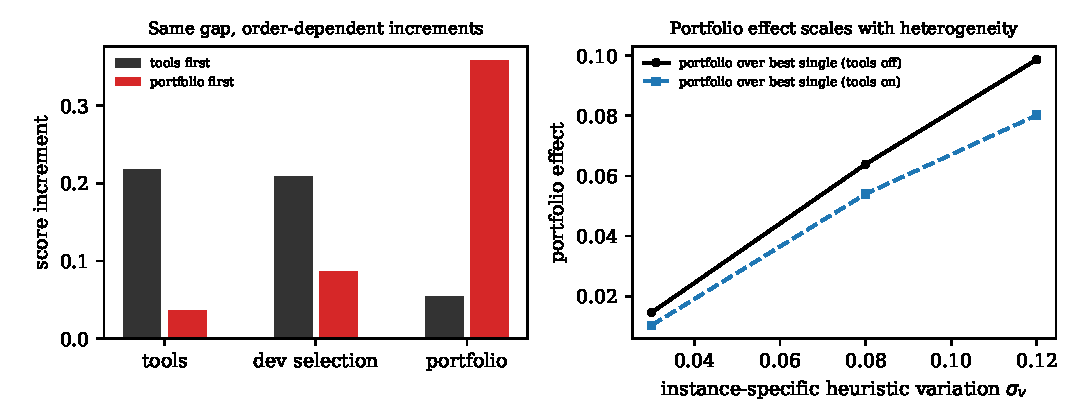
\includegraphics[width=\textwidth]{fig_attrib.pdf}
\caption{Toy model. Left: increments credited to each factor when they are added in two different orders, $\sigma_v=0.08$. Right: the portfolio effect (portfolio over the best single program) as the instance-specific variation $\sigma_v$ increases.}
\label{fig:attrib}
\end{figure}

The right panel of Figure~\ref{fig:attrib} shows the second point. The gain of a ten-program portfolio over the best single program is $0.010$ (tools on) at $\sigma_v=0.03$, $0.054$ at $0.08$ and $0.080$ at $0.12$. With tools absent the corresponding numbers are $0.014$, $0.063$ and $0.099$. The portfolio effect is governed by how much programs differ in which instances they handle well, a property of the problem family and generator, and an effect of about $0.10$ in the paper's own ablation is in the range an ordinary amount of instance-level variation produces. It is not evidence about the interface.

\section{What the reported numbers allow}

Three observations follow from the numbers in the paper itself, with the caveat that they come from different aggregations and are not exactly comparable.

\paragraph{Portfolio size alone is worth about as much as the margin over the strongest baseline.} The portfolio ablation reports $0.80$--$0.88$ per family at $n=1$ and $0.90$--$0.99$ at $n=10$, a difference of about $0.10$. The margin of the framework over the strongest language-model baseline is $0.075$ ($0.945$ against $0.870$). If the framework with $n=1$ is scored under the protocol of the baselines, which run one program, its score may be close to that of the strongest baseline, though per-family ranges and an overall mean cannot be compared exactly. The relevant table is not reported, and it is the table that would show whether the framework leads when the number of programs executed per instance is equal.

\paragraph{The gap from direct prompting is not apportioned.} The $0.571$ figure is taken from the benchmark's report, and the paper does not state how many samples or what selection that arm used. A bare model given $70$ samples, development-set selection and the ten-program test-time portfolio is the comparison that isolates the interface. The toy model's cell $(0,1,1)$ gives $0.937$ against $0.493$ for $(0,0,0)$, and so a large fraction of the gap can arise with no interface at all. The real figure is an empirical matter.

\paragraph{The four new problems are scored against a reference that includes the method.} For the four new problems the reference value is the best objective achieved on each instance by any method compared in the relevant figure, which includes the framework and its tuned metaheuristic competitors. Scores of $0.97$--$0.99$ therefore measure closeness to the best of the compared methods on each instance, and the framework's best-of-ten selection helps set that reference. The scores are informative about the comparison with the metaheuristics, and they are bounded by one by construction. The five baselines that produce no feasible program receive zero on these problems, which shows a difference in feasibility. The most likely contributor to that difference is the tool library, which supplies verified feasibility logic that the baselines must derive for themselves, and the paper's ablation of failure rate against the number of tools points the same way. The ablation reports failure rate and not score.

\section{Variance and units}

The framework's score of $0.945$ is reported without an interval, and the five-seed box plots are reported for the four new problems only. The paper states this limitation itself: variance across backbones, families and seeds has not been systematically modelled. For the 36 benchmark problems, the natural unit of replication is the problem, and a paired comparison across problems, with an interval, would show whether the margin over the strongest baseline is distinguishable from heterogeneity across problems. The earlier essay on paired inference sets out why a small number of problems with a shared difficulty structure calls for a paired design and an interval on the difference, and not for overlap of the marginal scores.

\section{Experiments that would support the sentence}

\begin{enumerate}
\item \textbf{Fill the factorial.} Run the baselines and the framework with factors toggled: tools on or off, development-set selection on or off, portfolio size from $1$ to $10$, including the bare model at the same candidate budget and test-time portfolio. Report all cells.
\item \textbf{Equalize test-time execution.} Compare the framework at $n=1$ with the single-program baselines, and compare the baselines allowed ten programs per instance with the framework at $n=10$.
\item \textbf{Report score and not only failure for the tools ablation.} The failure-rate curve against $K$ is informative; the score curve completes it.
\item \textbf{Report the interval over problems.} Present per-problem paired differences between the framework and each baseline, with an interval across the 36 problems.
\item \textbf{State what the reference includes.} For problems where the reference is the best of the compared methods, report scores against an independent reference as well, such as a long-run solver.
\end{enumerate}
If the framework's advantage persists in cells with equal test-time execution, the sentence locating the gain in the interface is supported and the framework earns it. If it shrinks, the finding is still valuable, since a portfolio of programs evolved on development instances is a useful engineering result, but it belongs to the search and not to the model-interface decomposition.

\section{Conclusion}

Holding the backbone fixed controls one source of variation and leaves several others free. The reported contrast changes the interface, the search budget, the use of development data, and the number of programs executed at test time together, and the portfolio effect and the tool effect interact, so the credit assigned to each factor depends on the order in which it is considered. The strengths of the study, a held-out test set, a matched generation budget, and an honest account of limitations, make the missing cells straightforward to add. Until they are, the defensible statement is that the combination of factors outperforms direct prompting and the strongest baseline, and that the share due to the interface in particular is not separated.

\begin{thebibliography}{9}
\bibitem[Gong et al.(2026)]{gong2026} Gong, H., Wang, S., Song, D., Sheu, J.-B., Yan, R. (2026). Large language models discover complementary heuristics for combinatorial optimization. \emph{Nature Machine Intelligence}. doi:10.1038/s42256-026-01307-8.
\end{thebibliography}

\end{document}
